\chapter{Marco Teórico}

En el presente capítulo se describen conceptos y patrones utilizados para el desarrollo del proyecto de pasantía, los cuales fueron seleccionados siguiendo los criterios de usabilidad, mantenibilidad, escalabilidad y portabilidad.

    \section{Modelo Vista Controlador (MVC)}
    
    El Modelo-Vista-Controlador es un patrón de arquitectura de \textit{software} que separa el modelo (objetos del negocio), la vista (interfaz con el usuario u otros sistemas) y el controlador (manejo de la información del negocio)\cite{MVC-tiw}.
    
    Técnicamente el usuario intereactúa con las vistas llenando formularios, solicitando información o simplemente haciendo algún \textit{click} que genere una petición al sistema. En ese momento es el controlador quien recibe la petición y genera las acciones necesarias sobre el modelo para así acceder a los datos y generar la nueva vista, resultado de la petición realizada y enviarla al usuario. Tal y como muestra la figura \ref{mvc-image}.
    
    \begin{figure}[htbp!] %Buscar imágen en español... -.-"
        \begin{center}
            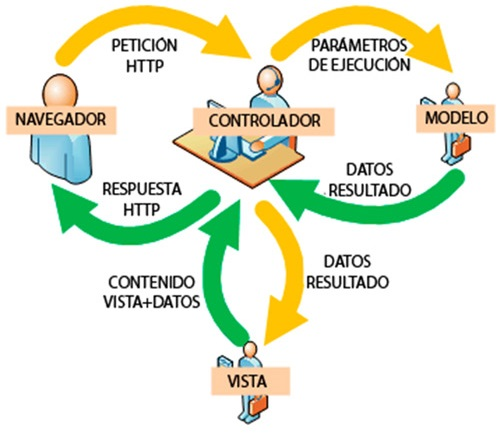
\includegraphics[width=.7\textwidth]{figures/mvc}
        \end{center}
        \caption{Representación gráfica del patrón Modelo Vista Controlador\cite{MVC-imagen}}
        \label{mvc-image}
    \end{figure}
    
    Específicamente, cada componente tiene una asignación independiente de los demás componentes. Estas son:
    
    \begin{enumerate}
        \item \textbf{Modelo}
            \begin{itemize}
                \item Almacenamiento de los datos.
                \item Estado del sistema.
                \item Recuperación de errores a nivel de datos.
            \end{itemize}
        \item \textbf{Vista}
            \begin{itemize}
                \item Presentación del modelo.
                \item Accede al modelo pero no puede cambiar su estado.
            \end{itemize}
        \item \textbf{Controlador}
            \begin{itemize}
                \item Reacciona a las peticiones del cliente.
                \item Comunica al modelo de las acciones ejecutadas.
                \item Direcciona a las vistas requeridas del lado del cliente.
            \end{itemize}
    \end{enumerate}
    
    Esto se busca, primordialmente, para hacer del código altamente mantenible en el tiempo, ya que antiguamente se realizaban los sistemas siguiendo lo que se conoce como \textit{``programación de espaguetti"} (programación no estructurada) la cual no llevaba una separación entre lo que era la vista y los procesos internos del sistema. Esto traía como consecuencia, en el momento de realizar algún cambio al sistema ya sea de formato o de interacción, que tuviera que modificarse integralmente vista, interacciones y (potencialmente) el modelo de datos.
    
    \section{Arquitectura Orientada a Servicios}
    \label{teorico-soa}
    
    Es una filosofía de desarrollo la cual actúa como una guía de diseño y facilita el mismo orientado a la escalabilidad del sistema, facilita las actualizaciones de uno o varios de los componentes MVC y minimiza el efecto que dicha actualización tiene sobre los demás.
    
    Según \citeauthor{SOA-libroGartner}\cite{SOA-libroGartner} y \citeauthor{SOA-tesis}\cite{SOA-tesis}, la incorporación de SOA empieza en las empresas hacia 2003, por las siguiente razones:
    
    \begin{itemize}
        \item La incesante presión de los negocios para la agilidad. Cuando una empresa quiere
        modificar sus procesos, productos o servicios, no puede permitirse el lujo de esperar por
        mucho tiempo. Debe ser posible cambiar la forma de aplicación de los sistemas de
        trabajo simplemente modificando los componentes que ya están en uso, en lugar de
        comprar o codificar nuevos componentes o sistemas enteros desde cero.
        
        \item La flexibilidad de la arquitectura SOA basada en Servicios Web de apoyo a múltiples
        aplicaciones.
        
        \item  La aceptación unánime de proveedores de los estándares de Servicios Web,
        especialmente de Simple Object Access Protocol (SOAP) y Web Service Description
        Language (WSDL)\cite{SOA-libroGartner}
        
    \end{itemize}
    
    SOA se basa en capas, cada una ofrece servicios a la siguiente y sus procedimientos internos se mantienen ocultos a las demás capas. Con esto se generan APIs de acceso estandarizado que son independientes de las tecnologías utilizadas en el desarrollo.
    
    En \citetitle{SOA-msdn}\cite{SOA-msdn} definen SOA usando el poema de Saxe sobre seis ciegos y un elefante.
    
    ``Seis ciegos de Indostan se encuentran con un elefante, cada uno describe el elefante de forma diferente porque se ve influenciado por sus propias experiencias (Ver figura \ref{elefante-saxe})
    
    \begin{itemize}
        \item Quien le toca la trompa cree que es una serpiente.
        \item Quien le toca los colmillos cree que son lanzas.
        \item Quien le toca las orejas cree que son abanicos.
        \item Quien le toca la panza cree que es una pared.
        \item Quien le toca la cola cree que es una cuerda.
        \item Quien le toca	las patas cree que son árboles."
    \end{itemize}
    

    \begin{figure}[htbp!]
        \begin{center}
            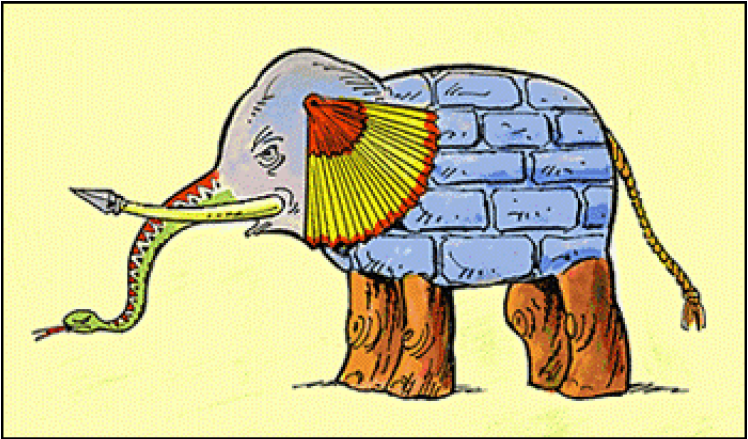
\includegraphics[width=.8\textwidth]{figures/Elefante}
        \end{center}
        \caption {El elefante de Saxe}
        \label{elefante-saxe}
    \end{figure}

    Se usa la analogía para ejemplificar el hecho de que haya varias definiciones diferentes de lo que es SOA en si, porque se le ha definido como patrón de diseño o como una filosofía de desarrollo, siendo esta última la definición adoptada para el trabajo descrito en el presente informe.
    
    También se puede usar dicha analogía para ejemplificar cómo los (potenciamente diversos) dispositivos pueden interactuar con el controlador y este a su vez con el modelo sin que ello represente un cambio fundamental en diseño o estructura de los mismos. Cada dispositivo interactúa con los servicios que necesita y más ningún otro.

%    \section{Autenticación}
    

    \section{Autenticación Basada en \textit{Tokens}}
    
    Autenticación, según se lee en \cite{AUTENTICACION-rae}, es la ``acción y efecto de autentificar". Esto es comprobar ante una autoridad la veracidad o legitimidad de un documento o un hecho\cite{AUTENTICACION-wordref}.
    
    En sistemas, el término es utilizado para definir el proceso de verificación de las credenciales de usuarios dentro de un sistema. Comunmente usando el par ``nombre de usuario" y ``contraseña" para ello.
    
    Existen diversos métodos para llevar a cabo la autenticación\cite{AUTENTICACION-aplicaciones}:
    
    \begin{enumerate}
        \item Sistemas basados en algo conocido, ya sea \textit{password} o \textit{passphrase}.
        \item Sistemas basados en algo poseído que puede ser un tarjeta de identidad o dispositivos USB.
        \item Sistemas basados en características físicas como voz, huellas dactilares o patrones oculares.
    \end{enumerate}
    
    La autenticación basada en \textit{tokens} es una forma de autenticación ligera que va de la mano con SOA, usa \textit{tokens} (o fichas) cifrados para la verificación de usuarios. Estas fichas son almacenadas en el cliente y enviadas en cada una de los \textit{requests} que realiza el navegador, la ficha es descifrada y se verifican las credenciales del usuario en cuestión\cite{TOKEN-tokenbasedauth}.
    
    Entre los datos almacenados en las fichas suelen estar:
    
    \begin{itemize}
        \item Nombre de usuario.
        \item Fecha de autenticación.
        \item Fecha de caducidad de la ficha.
    \end{itemize}

    Estas son cifradas en el servidor bajo una clave secreta elegida por el mismo servidor y que se usa para el posterior descifrado de las fichas.
    
    Aunque no es un determinante, es deseable que la ficha contenga suficiente información del usuario para poder indentificarlo en cada una de las solicitudes y además sea lo suficientemente ligera como para no afectar la carga de datos. Todo esto permite que el servidor no se sobrecargue con variables de estado o de sesión por cada usuario autenticado en un momento dado y además permite la portabilidad desesada para el sistema.
    
    En la figura \ref{tba-request} se especifican los pasos básicos de la autenticación basada en \textit{tokens}:% y \ref{tba-server}.
    
    \begin{enumerate}
        \item El cliente hace una solicitud de autenticación enviando en la solicitud el nombre de usuario (\textit{username}) y su contraseña (\textit{password}).
        \item El servidor, una vez procesadas y confirmadas las credenciales del usuario, envía el \textit{token} cifrado de regreso para que sea almacenado en el cliente.
        \item El cliente envía una solicitud de lo que sería una página de ``inicio" dentro del sistema, adjuntando entre los encabezados (\textit{headers}) de dicha solicitud, el \textit{token} almacenado.
        \item El servidor, en caso de confirmar el \textit{token}, responde con la página y acciones solicitadas.
    \end{enumerate}
    
    \begin{figure}[htbp!]
        \begin{center}
            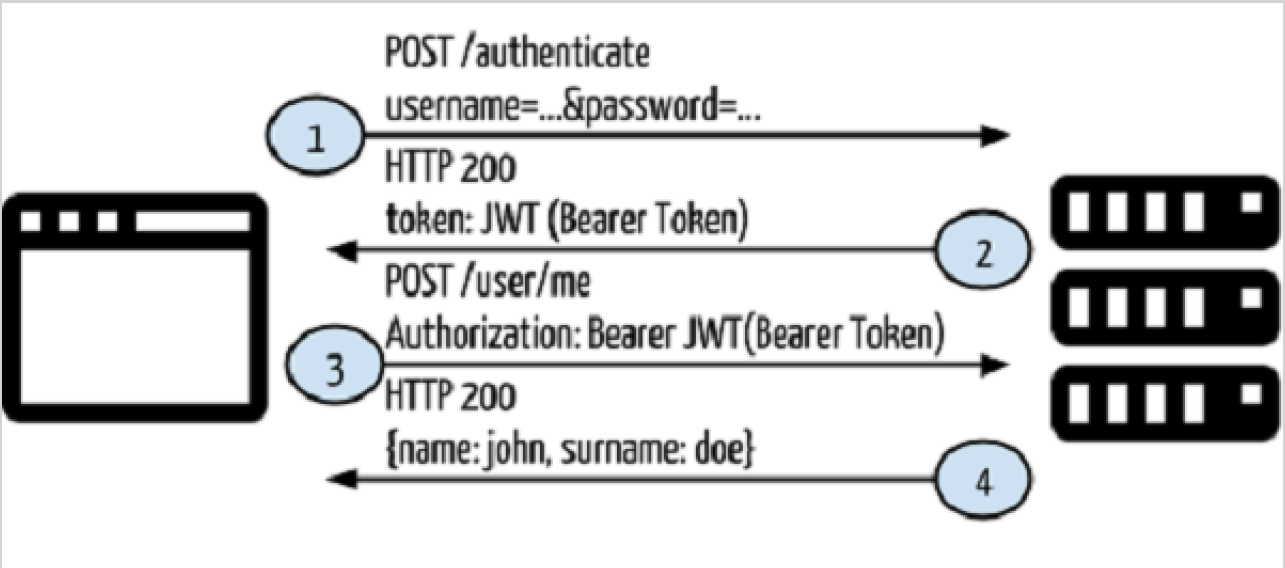
\includegraphics[width=.7\textwidth]{figures/tokenbarequest}
        \end{center}
        \caption{Autenticacion basada en fichas.}
        \label{tba-request}
    \end{figure}
    
    En adelante, y hasta que se complete el cierre de sesión, todas las solicitudes realizadas al servidor deben llevar adjunto el \textit{token} asignado para ser revisado en el servidor.
    
    En caso de fallos de autenticación, ya sea por credenciales incorrectas o un \textit{token} inválido, el servidor responderá con un mensaje de error y redireccionará la navegación a la vista de ``inicio de sesión" u otra página por defecto.
    
%    \begin{figure}[htbp!]
%        \begin{center}
%            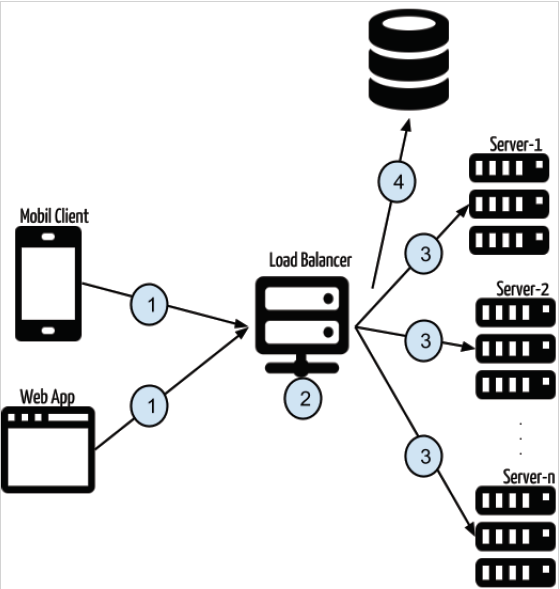
\includegraphics[width=.7\textwidth]{figures/tokenbaservers}
%        \end{center}
%        \caption{Portabilidad de la Autenticación Basada en Fichas.}
%        \label{tba-server}
%    \end{figure}
    
    \section{Inversión de Control}
    
    Concepto utilizado por primera vez por Martin Fowler\cite{IOC-dgarcia} que define una diferenciación principal entre un \textit{framework} y una biblioteca, siendo la biblioteca un conjunto de clases y funciones que pueden ser llamadas por el programa desarrollado y el \textit{framework} un diseño que controla el flujo y eventualmente llamará al código desarrollado para cumplir con las funciones específicas. De esta forma, el control de flujo no lo tiene el código si no el \textit{framework}, que responde a las solicitudes de los usuarios y solicita al programa las acciones requeridas.
    
    En este sentido, Spring cumple la cunción de manejar las solicitudes que surgen del \textit{front end} e invoca las secciones de código designadas como ``controladores" las cuales dependen (ver \ref{teorico-di}) de ``servicios".
    
    \section{Inyección de Dependencias}
    \label{teorico-di}
    
    Es una forma de IOC, se basa en que una clase A ``inyecte" objetos en otra clase B, siendo B dependiente de A, en lugar de permitir que la clase B se encargue de crear los objetos en sí misma\cites{IOC-mpachano}{IOC-dgarcia}.
    
    De esta forma se pueden crear objetos de una clase B y pasar el objeto de la clase A como argumento en el constructor de B o en algún \textit{setter} asignado al atributo. En adelante, cualquier función o procedimiento que precise información de A puede ser invocado a través de B aunque la responsabilidad de ejecución recaen en el objeto A.
    
    De forma más abstracta, se puede utilizar lo que en Java se conoce como \textit{interface} para dejar mayor margen a las modificaciones que puedan surgir con el tiempo en el código o en los requerimientos.
    
    En el caso de Spring, se usa inyección de dependencias en varios niveles:
    
    \begin{enumerate}
        \item Los ``controladores" utilizan a los ``servicios", que son interfaces creadas para realizar el procesamiento interno de los datos que llegan al servidor. Estas interfaces tienen procedimientos prederterminados, como toda ``interface", sus implementaciones deben implementar individualmente todos estos procedimientos y son inyectados (los ``servicios") en sus respectivos ``controladores".
        
        \item Los ``servicios" a su vez hace uso de los diferentes ``repositorios". También son interfaces que están estipuladas por JPA e implementadas por Hibernate (ver puntos \ref{tecno-jpa} y \ref{tecno-hibernate}) que son inyectados en los ``servicios" que así lo requieran.
    \end{enumerate}
    
\pagebreak